\documentclass[a4paper]{article}

\usepackage[T1]{fontenc}
\usepackage{textcomp}
\usepackage[english]{babel}
\usepackage{hyperref}
\usepackage{amsmath, amssymb, amsthm}
\usepackage{geometry}
\usepackage{tikz-cd}
\usepackage{subcaption}

% for including julia code
\usepackage{jlcode}

% Remove indentation globally
\setlength{\parindent}{0pt}
% Have blank lines between paragraphs
\usepackage[parfill]{parskip}

\hypersetup{
    colorlinks = true, % links instead of boxes
    urlcolor   = cyan, % external hyperlinks
    linkcolor  = blue, % internal links
    citecolor  = cyan   % citations
}

\newcommand{\R}{\mathbb{R}}
\newcommand{\C}{\mathbb{C}}
\newcommand{\Q}{\mathbb{Q}}
\newcommand{\N}{\mathbb{N}}
\newcommand{\A}{\mathbb{A}}
\newcommand{\Z}{\mathbb{Z}}

% use bullets for items
\renewcommand{\labelitemii}{$\circ$}
\renewcommand{\Im}{\operatorname{Im}}

\newcommand\numberthis{\addtocounter{equation}{1}\tag{\theequation}}

\newtheorem{theorem}{Theorem}[section]
\newtheorem{lemma}{Lemma}[section]

\theoremstyle{definition}
\newtheorem{definition}{Definition}[section]

\theoremstyle{definition}
\newtheorem{example}{Example}[section]

\theoremstyle{remark}
\newtheorem*{remark}{Remark}

\theoremstyle{definition}
\newtheorem{exercise}{Esercizio}[section]
\newtheorem*{exercise*}{Esercizio}

\begin{document}
\begin{titlepage}
    \begin{sffamily}
        \begin{large}
            \begin{center}
                \vbox to 100pt{%
                    
\includegraphics[width=3cm]{cherubino}%
                \vfil}
            \end{center}
            \begin{center}
                \begin{Large}
                    \uppercase{Universit\`a degli studi di Pisa}
                \end{Large}\\
                \rule{9cm}{.4pt}\\
                \smallskip
                Dipartimento di Matematica\\
                \medskip
                Corso di Laurea Triennale in
                Matematica\\
                \bigskip\vfill
                \begin{Large}
                    Laboratorio Computazionale
                \end{Large}\\
                \bigskip\bigskip\vfil
                \begin{Huge}
                    Parallel Homotopy Continuation in Julia
                \end{Huge}
                \bigskip\vfill
                \begin{tabular}{ll}
                    \textbf{Studente:} & Francesco Minnocci\\
                    \textbf{Matricola:} & 600455
                \end{tabular}
            \end{center}
            \begin{center}
                \vfill
                \rule{9cm}{.4pt}\\
                \medskip
                \uppercase{Anno Accademico 2022 - 2023}\\
            \end{center}
        \end{large}
    \end{sffamily}
\end{titlepage}

\tableofcontents
\newpage

\section{Introduction}
Homotopy Continuation is a numerical method for solving systems of polynomial equations.
It is based on the idea of ”deforming” a given system of equations into a simpler one, whose
solutions are known, and then tracking the solutions of the original system as the deformation
is undone.

In this project, the method will be implemented in the Julia programming language, making use
of parallel computing in order to speed multiple root finding. The method is described in detail
in \cite{BertiniBook}, which was the primary source for this report.

\section{Homotopy Continuation}
We will only consider \textit{square} systems of polynomial equations, i.e. systems of $n$ polynomial equations in $n$ variables, although or over- or under-determined systems can
often be solved by reducing them to square systems, by respectively choosing a suitable square subsystem or adding equations. Morever, we will restrict ourselves to systems with
isolated solutions, i.e. zero-dimensional varieties.

There are many ways to choose the "simpler" system, from now on called a \textit{start system}, but in general we can observe that, by Bezout's theorem, a system
$F=(f_1,\ldots,f_n)$ has at most $D:=d_1\ldots d_n$ solutions, where $d_i$ is the degre of $f_i(x_1,\ldots,x_n)$. So, we could build a start system of the same size and whose
polynomials have the same degrees, but whose solutions are easy to find, and thus can be used as starting points for the method.

For instance, the system $G=(g_1,\ldots g_n)$, where
$$ g_i(x_1,\ldots x_n)=x_i^{d_i}-1 ,$$
is such a system, since it has exactly the $D$ solutions
$$ \left\{\left(e^{\frac{k_1}{d_1}2\pi i},\ldots,e^{\frac{k_n}{d_n}2\pi i}\right),\text{ for }0\leq k_i\leq d_i-1\,\text{ and }i=1,\ldots,n\right\} .$$
\subsection{Choosing the homotopy}
The deformation between the original system and the start system is a \textit{homotopy}, for instance the convex combination of $F$ and $G$
\begin{equation}\label{eq:h1} H(x,t)=(1-t)F(x)+tG(x) ,\end{equation}
where $x:=(x_1,\ldots,x_n)$ and $t\in[0,1].$ This is such that the roots of $H(x,0)=G(x)$ are known, and the roots of $H(x,1)=F(x)$ are the solutions of the original system. Therefore, we can implicitly
define a curve $z(t)$ in $\C^n$ by the equation \begin{equation}\label{eq:h2} H(z(t),t)=0,\end{equation} so that in order to approximate the roots of $F$ it is enough to numerically track $z(t)$.

To do so, we derive the expression \eqref{eq:h2} with respect to $t$, and get the \textit{Davidenko Differential Equation}
$$ \frac{\partial H}{\partial z}\frac{\mathrm{d} z}{\mathrm{d} t}+\frac{\partial H}{\partial t}=0 ,$$
where $\frac{\partial H}{\partial z}$ is the Jacobian matrix of $H$ with respect to $z$:
$$
\frac{\partial H}{\partial z}=
\begin{pmatrix}
    \frac{\partial H_1}{\partial z_1} & \cdots & \frac{\partial H_1}{\partial z_n}\\
    \vdots & \ddots & \vdots\\
    \frac{\partial H_n}{\partial z_1} & \cdots & \frac{\partial H_n}{\partial z_n}
\end{pmatrix} .
$$
This can be rewritten as
\begin{equation}\label{eq:dav} \dot{z}=-\frac{\partial H}{\partial z}^{-1}\frac{\partial H}{\partial t} .\end{equation}
This is a system of $n$ first-order differential equations, which can be solved numerically for $z(t)$ as an initial value problem, and is called \textit{path tracking}.
\subsubsection{Gamma trick}
While \eqref{eq:h1} is a fine choice of a homotopy, it's not what it's called a \textit{good homotopy}: in order to ensure that the solution paths $z(t)$ for different roots
\begin{itemize}
    \item have no singularities, i.e. never cross each other for $t>0$ (at $t=0$, $F$ could have singular solutions), and
    \item don't go to infinity for $t\to 0$ ($F$ could have a solution at infinity),
\end{itemize}
we can employ the \textit{Gamma trick}: this consists in modifying the linear homotopy
\eqref{eq:h1} by susbtituting the parameter $t\in[0,1]$ with a complex curve $q(t)$ connecting $0$ and $1$:
$$ q(t)=\frac{\gamma t}{\gamma t+(1-t)} ,$$
where $\gamma\in(0,1)$ is a random complex parameter.This "probability one" procedure, i.e. for any particular system choosing $\gamma$ outside of a finite amount of lines through
the origin ensures that we get a good homotopy, basically because of the finiteness of the branch locus of the homotopy.
After substituting, we get
$$ H(x,t)=\frac{(1-t)}{\gamma t+(1-t)}F(x)+\frac{\gamma t}{\gamma t+(1-t)}G(x) ,$$
and clearing denominators, here's our final homotopy:
\begin{equation}\label{eq:h3} H(x,t)=(1-t)F(x)+\gamma tG(x) .\end{equation}
\subsection{Tracking down the roots}
We now want to track down individual roots, following the solution paths from
a root $z_0$ of the start system by solving the initial value problem associated to the Davidenko differential equation \eqref{eq:dav} with starting value $z_0$ and
$t$ ranging from $1$ to $0$.

This will be done numerically, using a first-order predictor-corrector tracking method, which consists in first using Euler's method to get an approximation
$\widetilde{z}_i$, and then using Newton's method to correct it
using equation \eqref{eq:h2} so that it becomes a good approximation $z_i$ of the next value of the solution path.
\subsubsection{Predictor: Euler's method}
Recall that Euler's method consists in approximating the solution of the initial value problem associated to a first-order ordinary differential equations
% Braced system of equations below
\begin{equation*}
    \left\{
        \begin{aligned}
            &\dot{z}=f(z,t)\\
            &z(t_0)=z_0
        \end{aligned}
    \right.
\end{equation*}
by the sequence of points $(z_i)_{i\in\N}$ defined by the recurrence relation
$$ z_{i+1}=z_i+h\cdot f(z_i,t_i) ,$$
where $h$ is the step size.
In our case, we have $$f(z,t)=-\left(\frac{\partial H}{\partial z}(z,t)\right)^{-1}\frac{\partial H}{\partial t}(z,t)$$ and $t_0=1$, since we track from $1$ to $0$. For the same
reason, we set $$t_{i+1}=t_i-h.$$
\subsubsection{Corrector: Newton's method}
Since we want to solve $$H(z,t)=0,$$ we can use Newton's method to improve the approximation $\widetilde{z_i}$ obtained by Euler's method to a solution of such equation.
This is done by moving towards the root of the tangent line of $H$ at the current approximation, or in other words through the iteration
$$ z_{i+1}=z_i-\left(\frac{\partial H}{\partial z}(z_i,t_{i+1})\right)^{-1}H(z_i,t_{i+1}) ,$$
where this time $z_0=\widetilde{z}_i$, with $\widetilde{z}_i$ and $t_{i+1}$ obtained from the $i$-th Euler step.

Usually, only a few steps of Newton's method are needed; we will use a fixed number of 5 iterations.
At this point, we use the final value of the Newton iteration as the starting value for the next Euler step.
\subsubsection{Adaptive step size}
In order to improve the efficiency of the method, we will use an adaptive step size, which will be based on the norm of the residual of the Newton iteration.
If the desired accuracy is not reached, for instance when the norm of $H(z_i,t_i)$ is bigger than $10^{-8}$,
then we halve the step size; if instead we have 5 "successful" iterations in a row, we double the step size.

\section{Parallelization}
\subsection{Multithreading}
When testing the method, we tried to use multithreading to speed up the computation.
This was done in Julia by using the \texttt{Threads.@threads} macro, which automatically distributes the work of a \texttt{for} loop among the available threads.
However, in the case of looping over multiple roots, this didn't improve the performance, as the overhead of the multithreading was too big compared to the actual computation time,
as the systems were too small to benefit from this kind of parallelization, as can be seen by the results in Appendix \hyperref[sec:mt]{B}.

\subsection{MPI}
Next, we tried to use MPI to parallelize the tracking of the roots.
This was done by using the \texttt{MPI.jl} package, which provides a Julia interface to the MPI library.

\section{Appendix A: Implementation}
\subsection{Julia code}
\jlinputlisting[caption={solve.jl}]{../solve.jl}
\jlinputlisting[caption={start-system.jl}]{../start-system.jl}
\jlinputlisting[caption={homotopy.jl}]{../homotopy.jl}
\jlinputlisting[caption={homogenize.jl}]{../homogenize.jl}
\jlinputlisting[caption={euler-newton.jl}]{../euler-newton.jl}
\jlinputlisting[caption={adapt-step.jl}]{../adapt-step.jl}
\jlinputlisting[caption={plot.jl}]{../plot.jl}
\subsection{Hardware}
\section{Appendix B: Results}

\subsection{Multithreading}\label{sec:mt}

Here are the plots for the solutions of four different 2x2 systems, with the single-threaded version next to the multithreaded one:

\newgeometry{left=.1cm,top=0.1cm}
\begin{figure}[htb]
    \begin{tabular}{c c c}
        \subcaptionbox{Single-threaded}{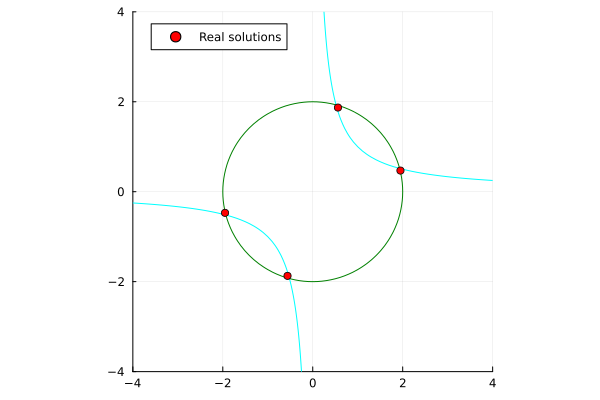
\includegraphics[width=0.45\textwidth]{../plots/solutions1.png}} &
        $\left\{\begin{aligned}
                    &x^3 + 5x^2 - y - 1 \\
                    &2x^2 - y - 1 \\
        \end{aligned}\right.$ &
        \subcaptionbox{Multithreaded}{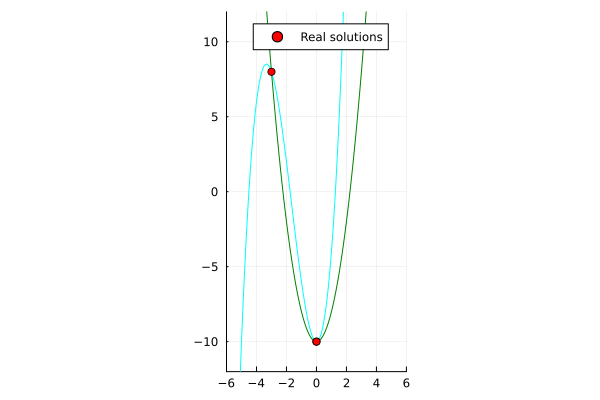
\includegraphics[width=0.45\textwidth]{../plots/solutions1_6.png}} \\
        \vspace{0.5cm} \\
        \subcaptionbox{Single-threaded}{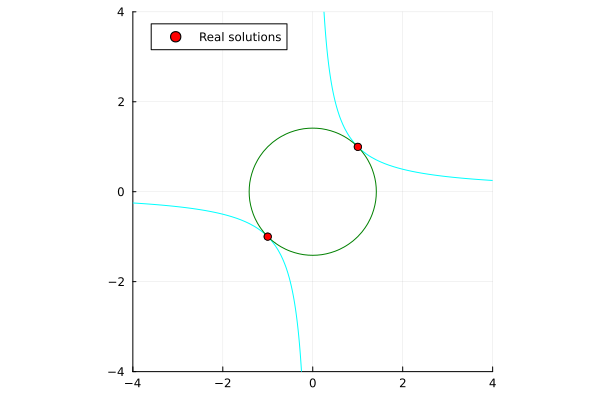
\includegraphics[width=0.45\textwidth]{../plots/solutions2.png}} &
        $\left\{\begin{aligned}
                    &x^2 + 2y  \\
                    &y - 3x^3 \\
        \end{aligned}\right.$ &
        \subcaptionbox{Multithreaded}{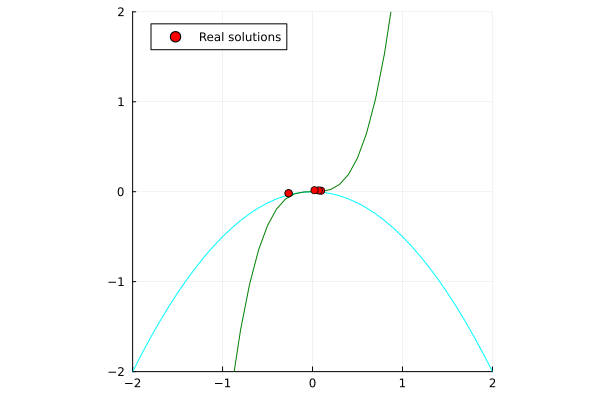
\includegraphics[width=0.45\textwidth]{../plots/solutions2_6.png}} \\
        \vspace{0.5cm} \\
        \subcaptionbox{Single-threaded}{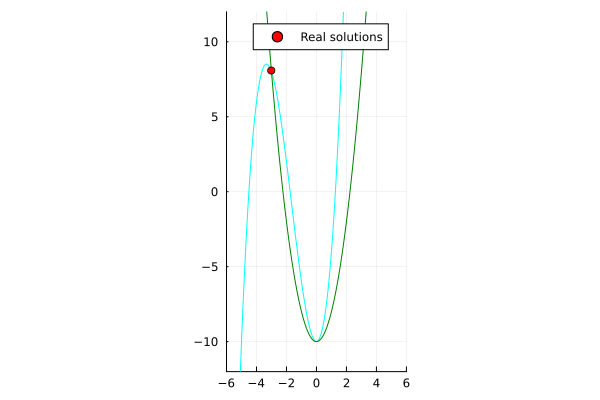
\includegraphics[width=0.45\textwidth]{../plots/solutions3.png}} &
        $\left\{\begin{aligned}
                    &x^2 + y^2 - 4 \\
                    &xy - 1 \\
        \end{aligned}\right.$ &
        \subcaptionbox{Multithreaded}{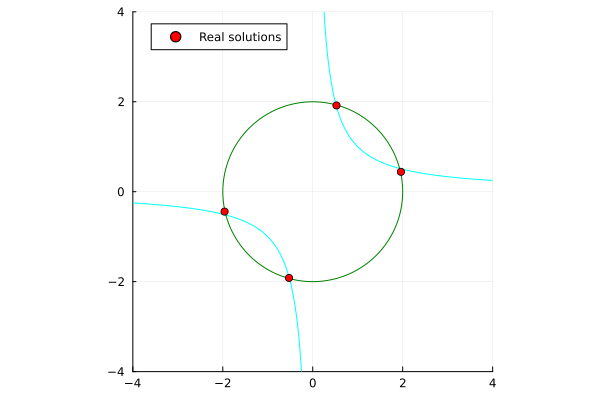
\includegraphics[width=0.45\textwidth]{../plots/solutions3_6.png}} \\
        \vspace{0.5cm} \\
        \subcaptionbox{Single-threaded}{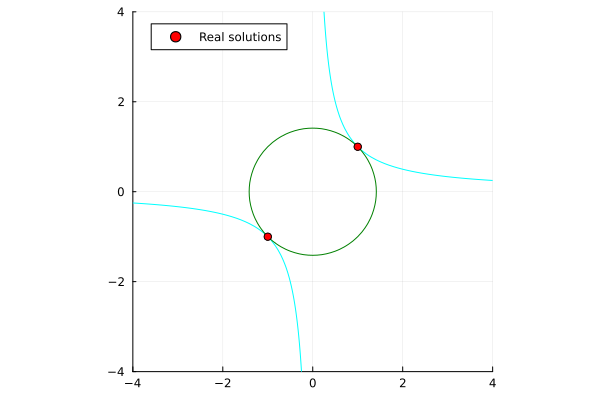
\includegraphics[width=0.45\textwidth]{../plots/solutions4.png}} &
        $\left\{\begin{aligned}
                    &x^2 + y^2 - 2 \\
                    &xy - 1 \\
        \end{aligned}\right.$ &
        \subcaptionbox{Multithreaded}{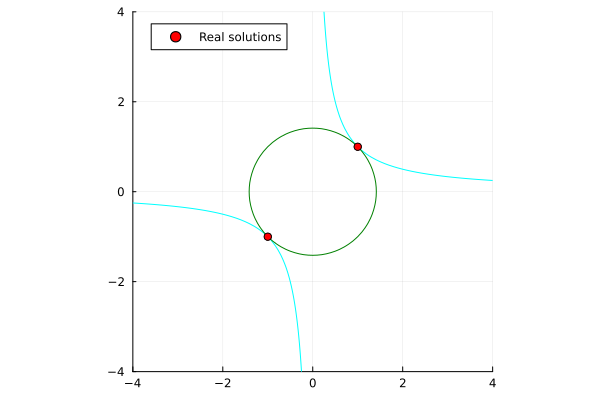
\includegraphics[width=0.45\textwidth]{../plots/solutions4_6.png}} \\
    \end{tabular}
\end{figure}

\restoregeometry

\thebibliography{2}
\bibitem{BertiniBook} Bates, Daniel J. \textit{Numerically solving polynomial systems with Bertini}. SIAM, Society for Industrial Applied Mathematics, 2013.
\end{document}
